\documentclass[palatino,nochap]{apuntes}

\title{Análisis de grafos de redes sociales}
\author{Daniel Ruiz Mayo, Alberto Javier Parramón, Víctor de Juan}
\date{}

% Paquetes adicionales

% --------------------

\begin{document}
\pagestyle{plain}
\maketitle

% Contenido.

%% Apéndices (ejercicios, exámenes)
%\appendix

\section{Ejecución}

Para ejecutar esta parte de la práctica únicamente hay que poner como directorio de trabajo el directorio de la práctica bmi1414-p4-12. Posteriormente habrá que ejecutar la clase AnálisisGrafos.java. El método main de dicha clase calcula todas las métricas que se piden en el enunciado y va informando paso por paso de las acciones realizadas. El proceso entero puede tardar cerca de 80 minutos.

Las gráficas se generan con R, los scripts R y las gráficas generados también vienen adjuntados en la práctica en el directorio $resultados/grados$, $resultados/prgrado$ y $resultados/betweenessgrado$.

Así mismo las salidas por fichero que se piden se encuentran en el directorio $resultados$.


\section{Análisis}

\textbf{TOP 10 PageRank de nodo:}
\begin{verbatim}
small2 3 0.23376623376623362
small1 6 0.108402068008146
small2 1 0.09577922077922071
small2 2 0.09577922077922071
small2 4 0.09577922077922071
small2 5 0.09577922077922071
small2 6 0.09577922077922071
small2 7 0.09577922077922071
small2 8 0.09577922077922071
small2 9 0.09577922077922071
\end{verbatim}


\textbf{TOP 10 coeficiente de clustering de nodo:}
\begin{verbatim}
fb 865 1.0
fb 868 1.0
fb 873 1.0
fb 877 1.0
fb 887 1.0
fb 888 1.0
fb 899 1.0
twitter envasados 1.0
fb 854 1.0
fb 851 1.0
\end{verbatim}


\textbf{TOP 10 arraigo de arcos:}
\begin{verbatim}
twitter e_463148-neilepstein-neilepstein 1.2
twitter e_267707-beaulebens-beaulebens 1.0363636363636364
fb e_644312-2824-3091 1.0
fb e_607521-3911-3700 1.0
fb e_607635-3849-3444 1.0
fb e_607522-3864-3813 1.0
fb e_560900-659-627 1.0
fb e_575932-135-309 1.0
fb e_560295-3127-3074 1.0
fb e_560369-195-78 1.0
\end{verbatim} 


\textbf{Coeficiente de clustering global de los grafos: }
\begin{verbatim}
small1 0.5641025641025641
small2 0.6243386243386244
twitter 0.2732562078881961
fb 0.5437268365614687
erdos 0.250008694894668
barabasi 0.14596066400839333
\end{verbatim}



\textbf{Coeficiente de asortatividad de los grafos: }
\begin{verbatim}
small1 -0.21153846153846154
small2 -0.3333333333333333
twitter -0.14680502816984128
fb 0.6299345168308577
erdos -0.0019803418041128957
barabasi -0.41012724063787015
\end{verbatim}


\textbf{Número de puentes locales: }

Como anecdota comentar que al encontrar puentes locales también hemos encontrado parejas de nodos comunicados entre sí y descomunicados del resto del grafo, por definición son puentes locales pero son muchos más raros que estos. Vemos aquí los puentes locales de cada red:
\begin{verbatim}
small1 5
small2 0
twitter 6843
fb 712
erdos 0
barabasi 1235
\end{verbatim}



\textbf{Paradoja de la amistad}
Para ver si se cumple la paradoja de la amistad hemos utilizado la siguiente fórmula:
$$ AVG_u g(u) \leq AVG_{u\rightarrow v}g(v) $$
\begin{verbatim}
small1: Sí se cumple la paradoja de la amistad: 2.769230769230769 <= 2.9102564102564097
small2: Sí se cumple la paradoja de la amistad: 3.5555555555555554 <= 4.481481481481482
twitter: Sí se cumple la paradoja de la amistad: 92.2125835078273 <= 237.10256141566012
fb: Sí se cumple la paradoja de la amistad: 42.55771659509977 <= 56.071613980320535
erdos: Sí se cumple la paradoja de la amistad: 499.713 <= 500.481589769589
barabasi: Sí se cumple la paradoja de la amistad: 4.761904761904762 <= 43.26991815460132
\end{verbatim}


\subsection{Representación gráfica de la distribución de grado }

\textbf{twitter:}

\begin{center}
	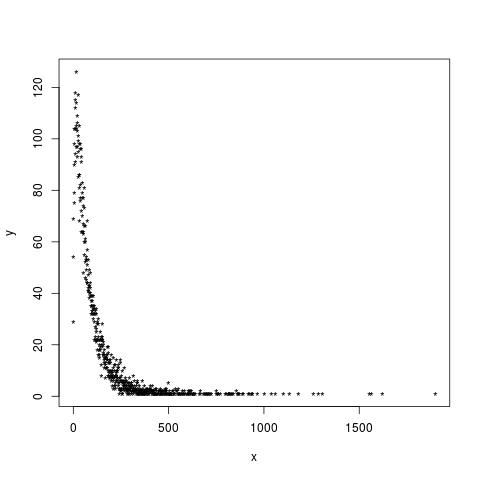
\includegraphics[scale=0.45]{img/twitter_grado}
\end{center}


\textbf{facebook:}

\begin{center}
	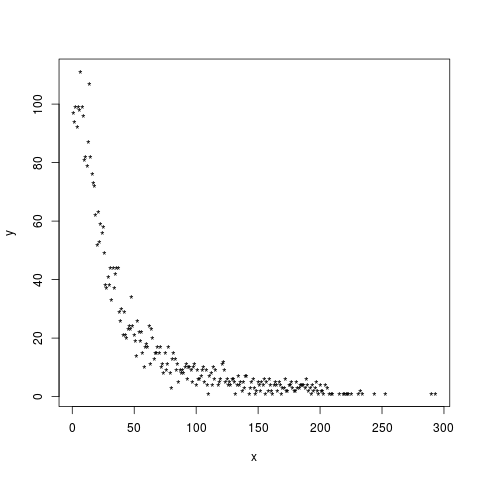
\includegraphics[scale=0.45]{img/fb_grado}
\end{center}


\textbf{barabasi:}

\begin{center}
	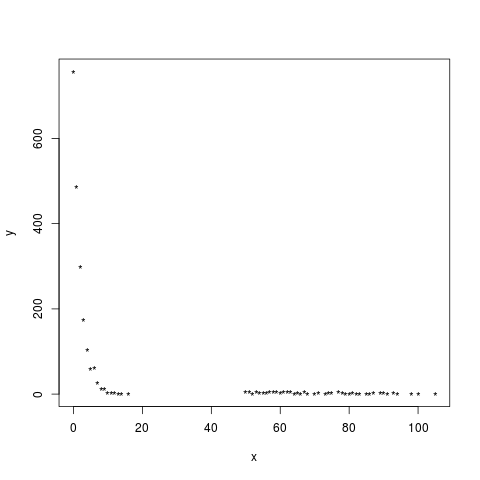
\includegraphics[scale=0.45]{img/barabasi_grado}
\end{center}


\textbf{erdos:}

\begin{center}
	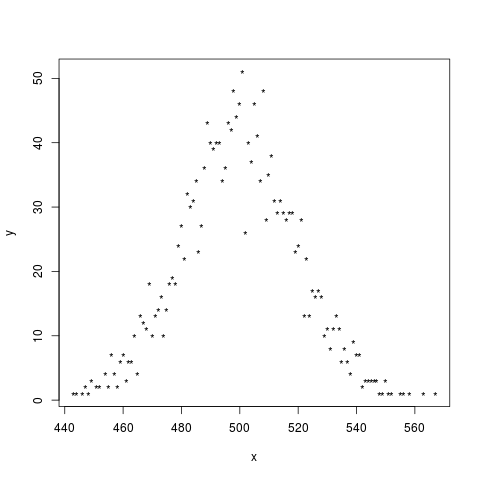
\includegraphics[scale=0.45]{img/erdos_grado}
\end{center}


\subsection{Representación gráfica del grado frente al PageRank }

\textbf{small1:}

\begin{center}
	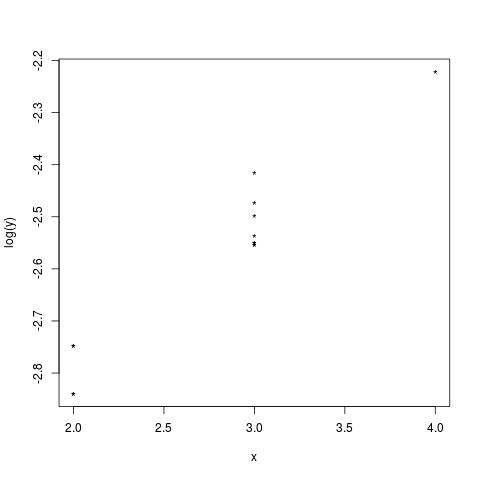
\includegraphics[scale=0.45]{img/small1_grado-pr}
\end{center}


\textbf{small2:}

\begin{center}
	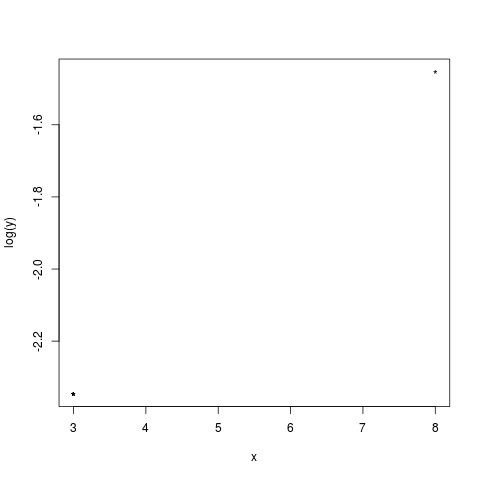
\includegraphics[scale=0.45]{img/small2_grado-pr}
\end{center}


\textbf{twitter:}

\begin{center}
	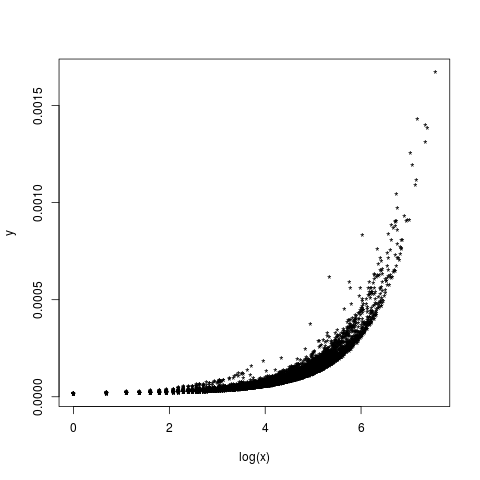
\includegraphics[scale=0.45]{img/twitter_grado-pr}
\end{center}


\textbf{facebook:}

\begin{center}
	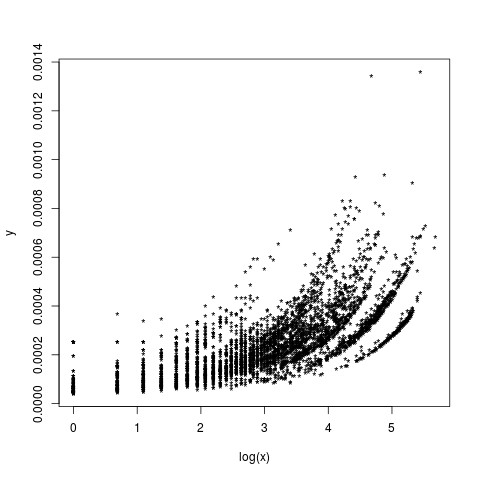
\includegraphics[scale=0.45]{img/fb_grado-pr}
\end{center}


\textbf{barabasi:}

\begin{center}
	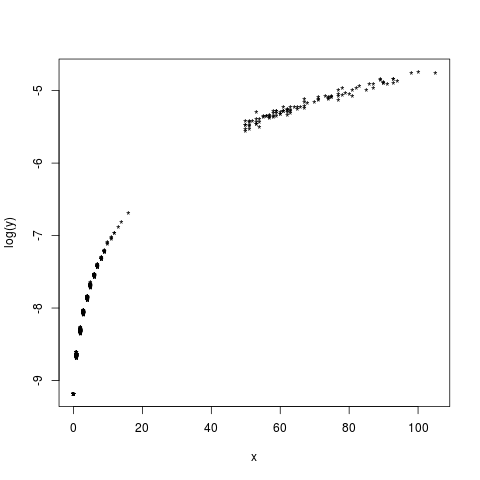
\includegraphics[scale=0.45]{img/barabasi_grado-pr}
\end{center}


\textbf{erdos:}

\begin{center}
	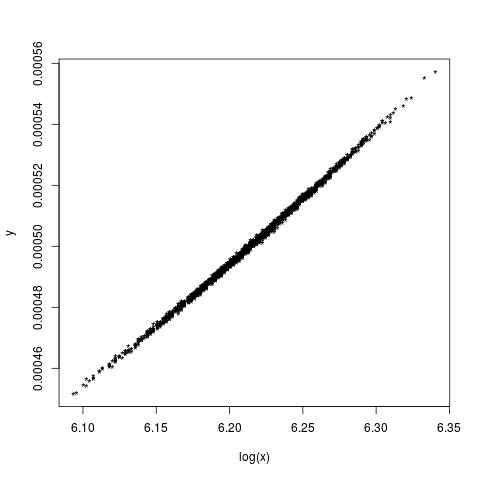
\includegraphics[scale=0.45]{img/erdos_grado-pr}
\end{center}


\subsection{Representación gráfica del grado frente al betweeness }

\textbf{small1:}

\begin{center}
	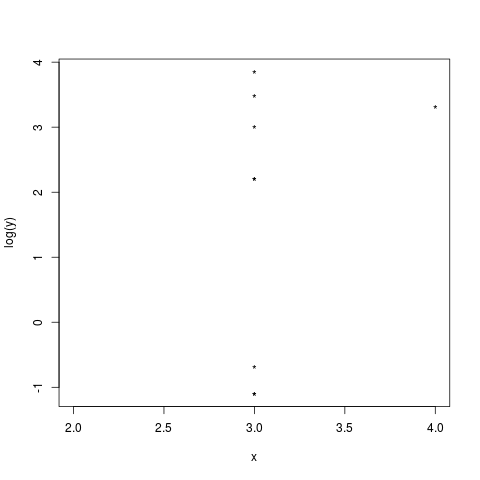
\includegraphics[scale=0.45]{img/small1_grado-betweeness}
\end{center}


\textbf{small2:}

\begin{center}
	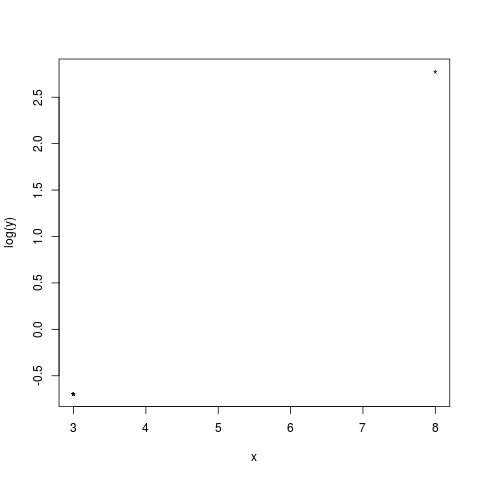
\includegraphics[scale=0.45]{img/small2_grado-betweeness}
\end{center}


\textbf{twitter:}

\begin{center}
	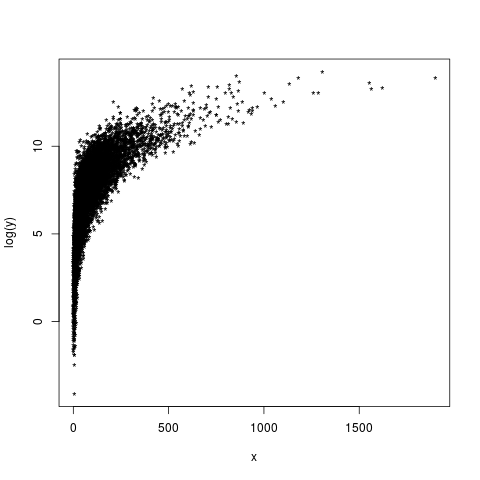
\includegraphics[scale=0.45]{img/twitter_grado-betweeness}
\end{center}


\textbf{facebook:}

\begin{center}
	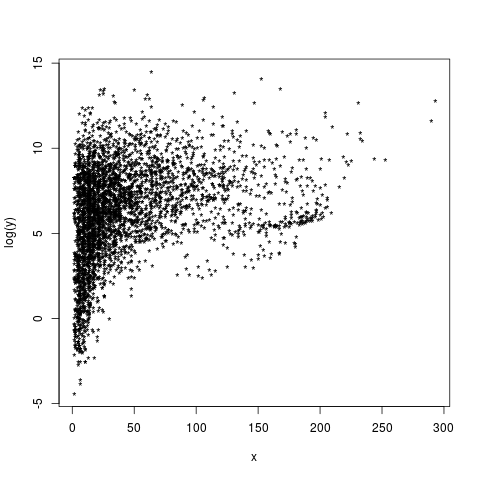
\includegraphics[scale=0.45]{img/fb_grado-betweeness}
\end{center}


\textbf{barabasi:}

\begin{center}
	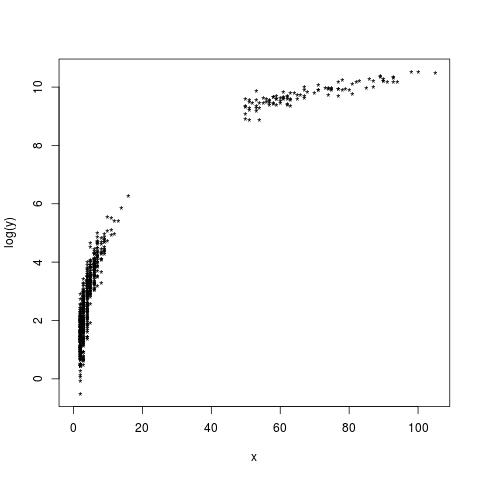
\includegraphics[scale=0.45]{img/barabasi_grado-betweeness}
\end{center}


\textbf{erdos:}

\begin{center}
	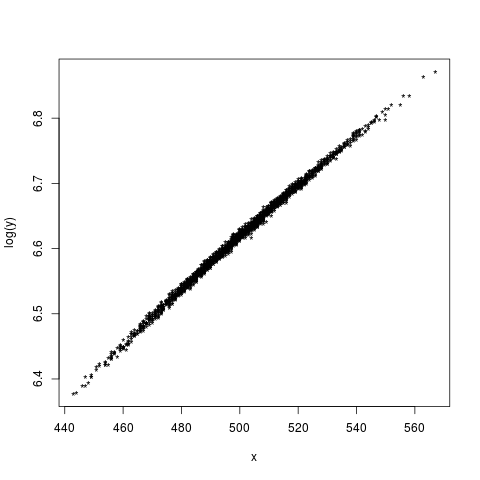
\includegraphics[scale=0.45]{img/erdos_grado-betweeness}
\end{center}

\end{document}
